\section{Single GPU algorithm} \label{oneGPU}

\subsection{Correction} \label{one_GPU:correct}
The KFBI method involves making corrections to each irregular node \cite{ying2007kernel}. Therefore, on a single GPU, each thread block is comprised of 1,024 threads, and each thread corresponds to precisely one irregular node for correction. 

Suppose that the rectangle domain $\mathcal{B}$ is partitioned into a uniform Cartesian grid with nodes $ \left\{\mathbf{p}_{i, j} :=\left(x_i, y_j\right): 0 \leq i \leq I, 0 \leq j \leq J\right\}$. For simplicity, assume the grid has the same spacing in the horizontal and vertical directions and denote by $h>0$ the spacing parameter, i.e., $h=x_{i+1}-x_i=y_{j+1}-y_j$. Let $v_{i,j} = v_{h}(\mathbf{p}_{i,j})$ be the finite difference approximation of $v(\mathbf{x})$ at the grid node $\mathbf{p}_{i, j}$.
One can describe the GPU version of the correction method as the following Algorithm $\ref{one_GPU:correction_algo}$ and schematic plot in Fig.\,$\ref{fig:One_GPU:irregular_node}$.
\begin{algorithm}
\renewcommand{\algorithmicrequire}{\textbf{Input:}}
\renewcommand{\algorithmicensure}{\textbf{Output:}}
\caption{Correction Procedure}
\begin{algorithmic}[1]
\Require $\text{intersection nodes, irregular nodes, } \Phi, \mathcal{F}$.
\Ensure $\text{corrected right hand side $\tilde{f}_{i,j}$ on each irregular nodes}$.
\State Locate index of irregular nodes by $\text{index} \xleftarrow[]{}$ blockIdx.x $\times$ blockDim.x + blockIdx.x
\State For irregular nodes $\mathbf{p}_{i,j}$, find the corresponding intersection nodes set $\mathcal{Q} = \left\{\mathbf{q}_{i_{1}}, \mathbf{q}_{i_{2}}, \cdots\right\}$
    \For {$\text{ each } \mathbf{q}_{i_{k}} \text{ in } \mathcal{Q}$}
    \State Interpolate $\Phi$ and calculate jumps of derivatives at of $\mathbf{q}_{i_{k}}$.
    \State  Evaluate and modify correction value $\tilde{f}_{i,j}$ by the discrete scheme on irregular nodes $\mathbf{p}_{i,j}$.
    \EndFor
\end{algorithmic}\label{one_GPU:correction_algo}
\end{algorithm}

\begin{figure}[htpt!]
    \centering
    \subfigure[Intersection nodes]{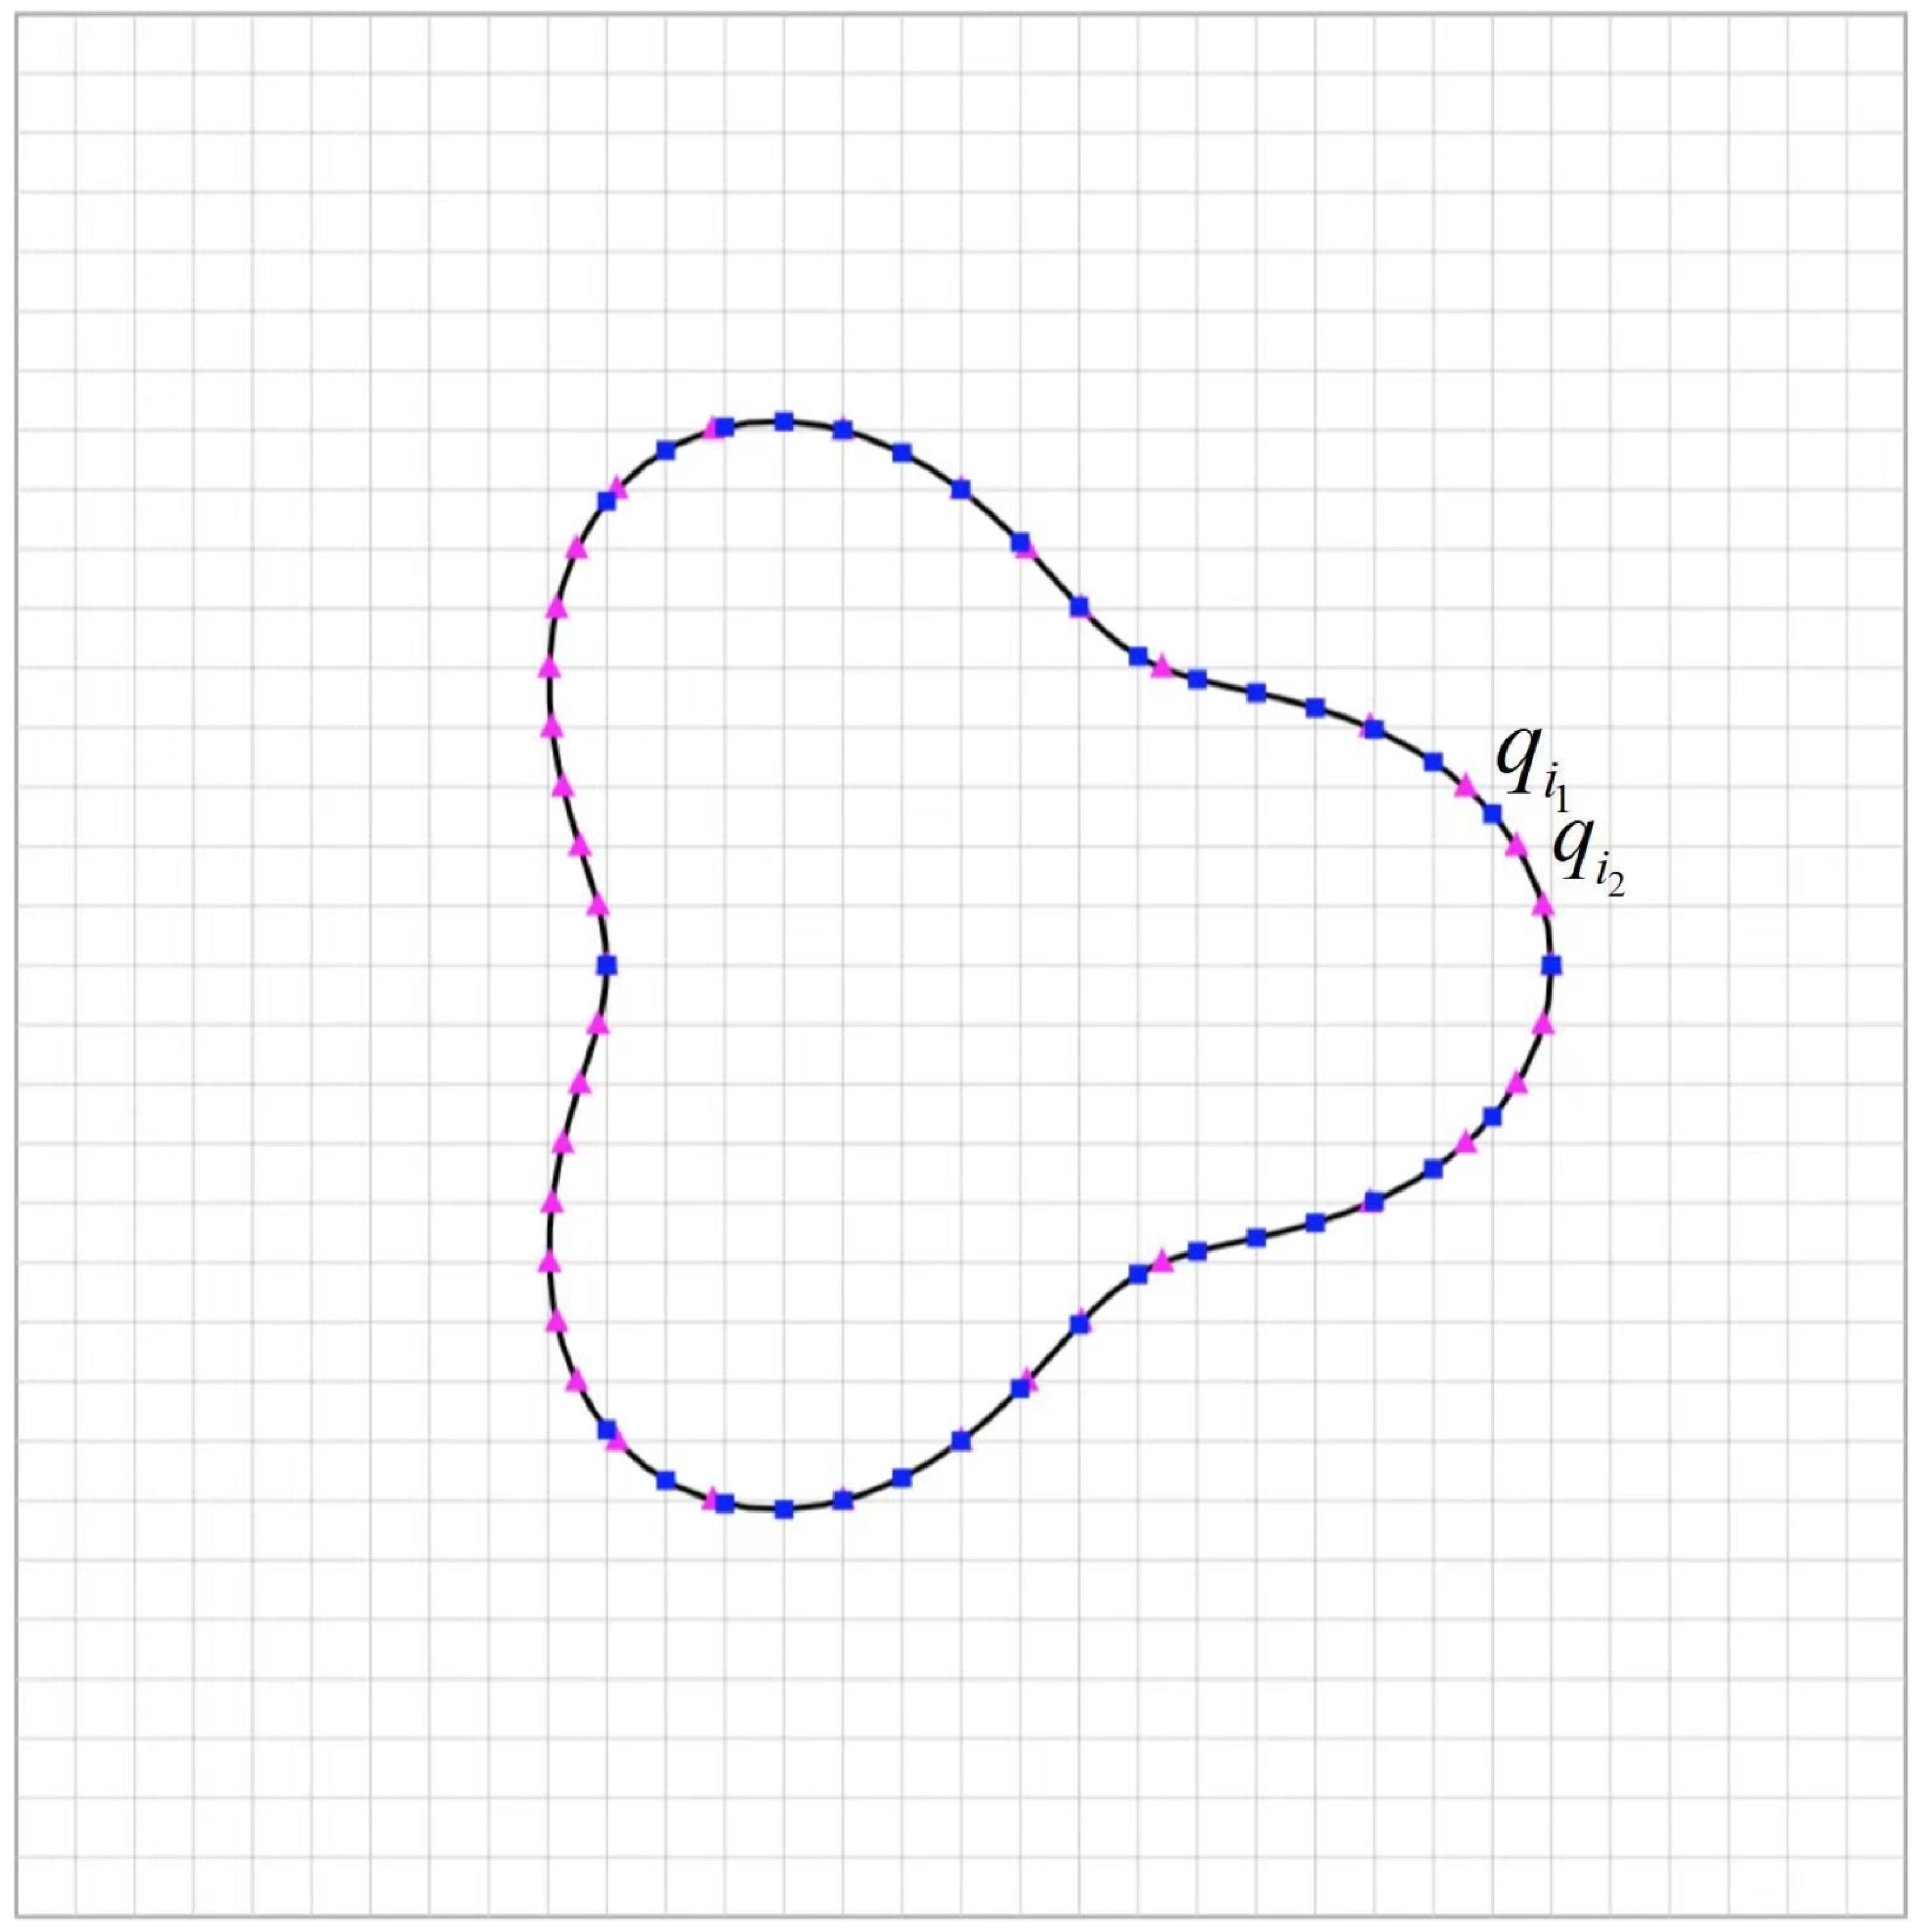
\includegraphics[width=0.35\textwidth]{figure/one_gpu_irregular_node.eps}\label{fig:oneGPU:intersect_node}}
    \subfigure[Irregular nodes]{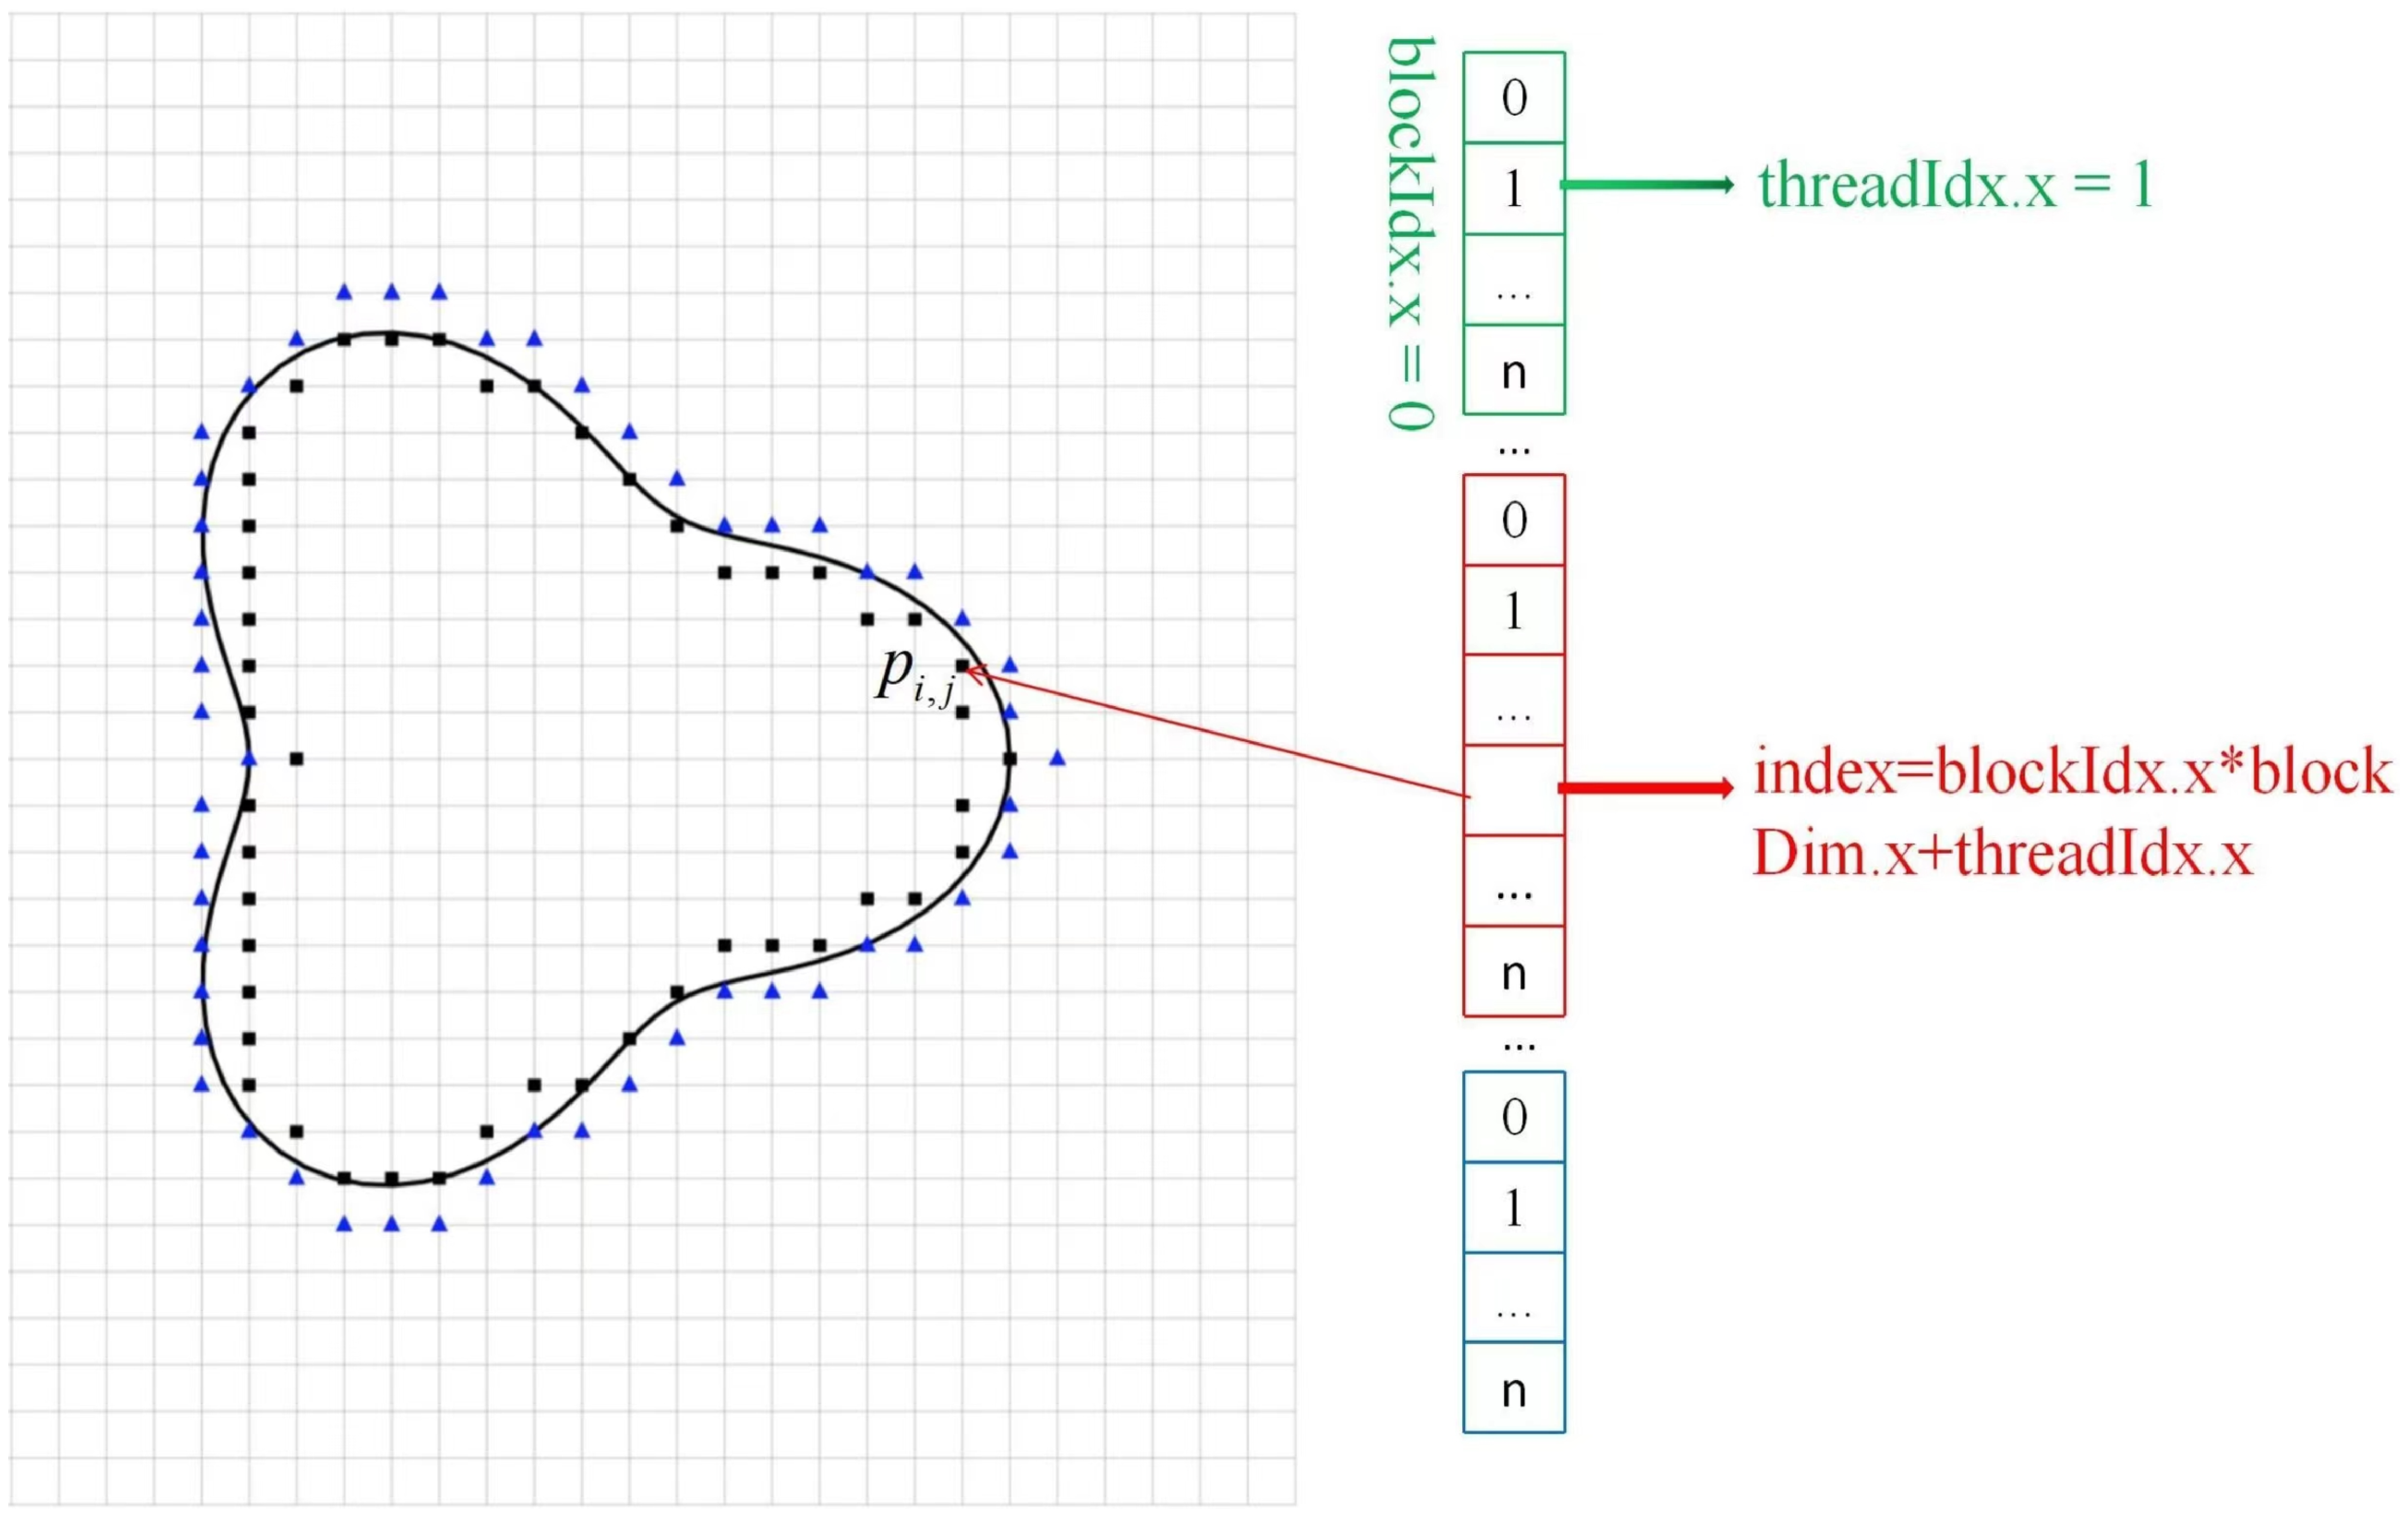
\includegraphics[width=0.55\textwidth, height=0.3501\textwidth]{figure/one_gpu_irregular_node_2.eps}\label{fig:oneGPU:irregular_node}}
    % \subfigure[Intersection nodes]{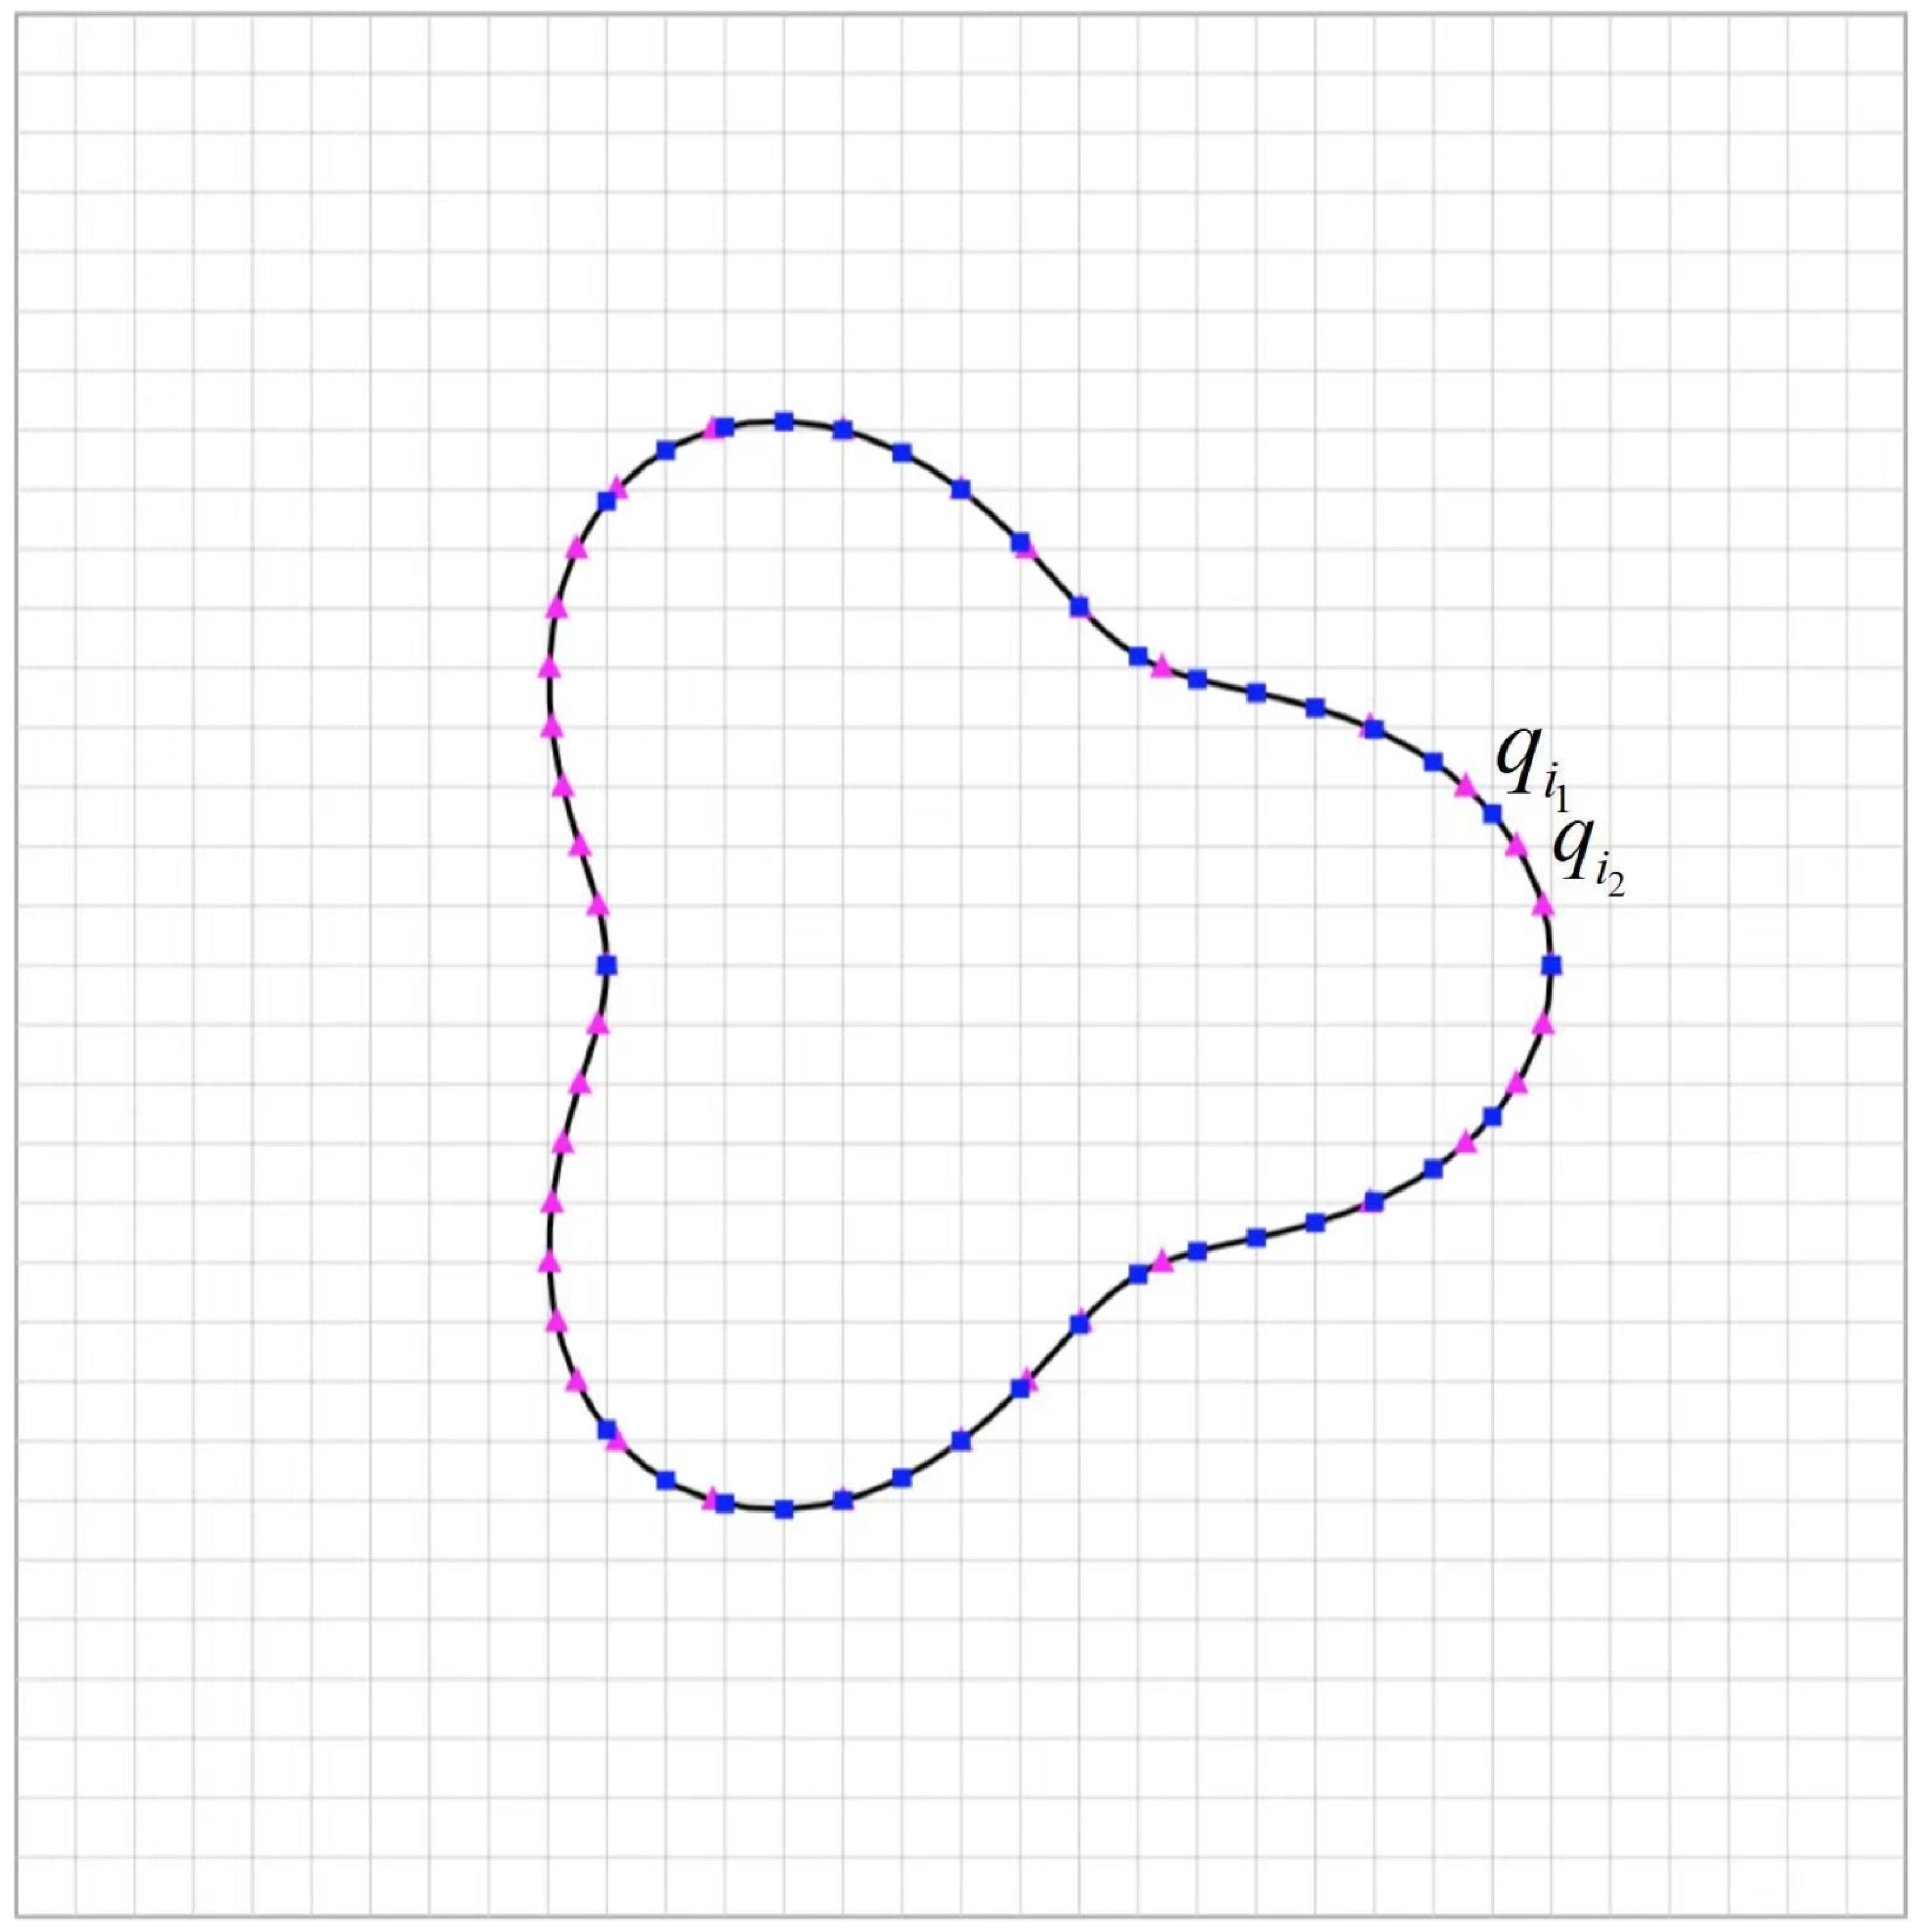
\includegraphics[width=0.4\textwidth]{figure/one_gpu_irregular_node.eps}\label{fig:oneGPU:intersect_node}}
    % \subfigure[Irregular nodes]{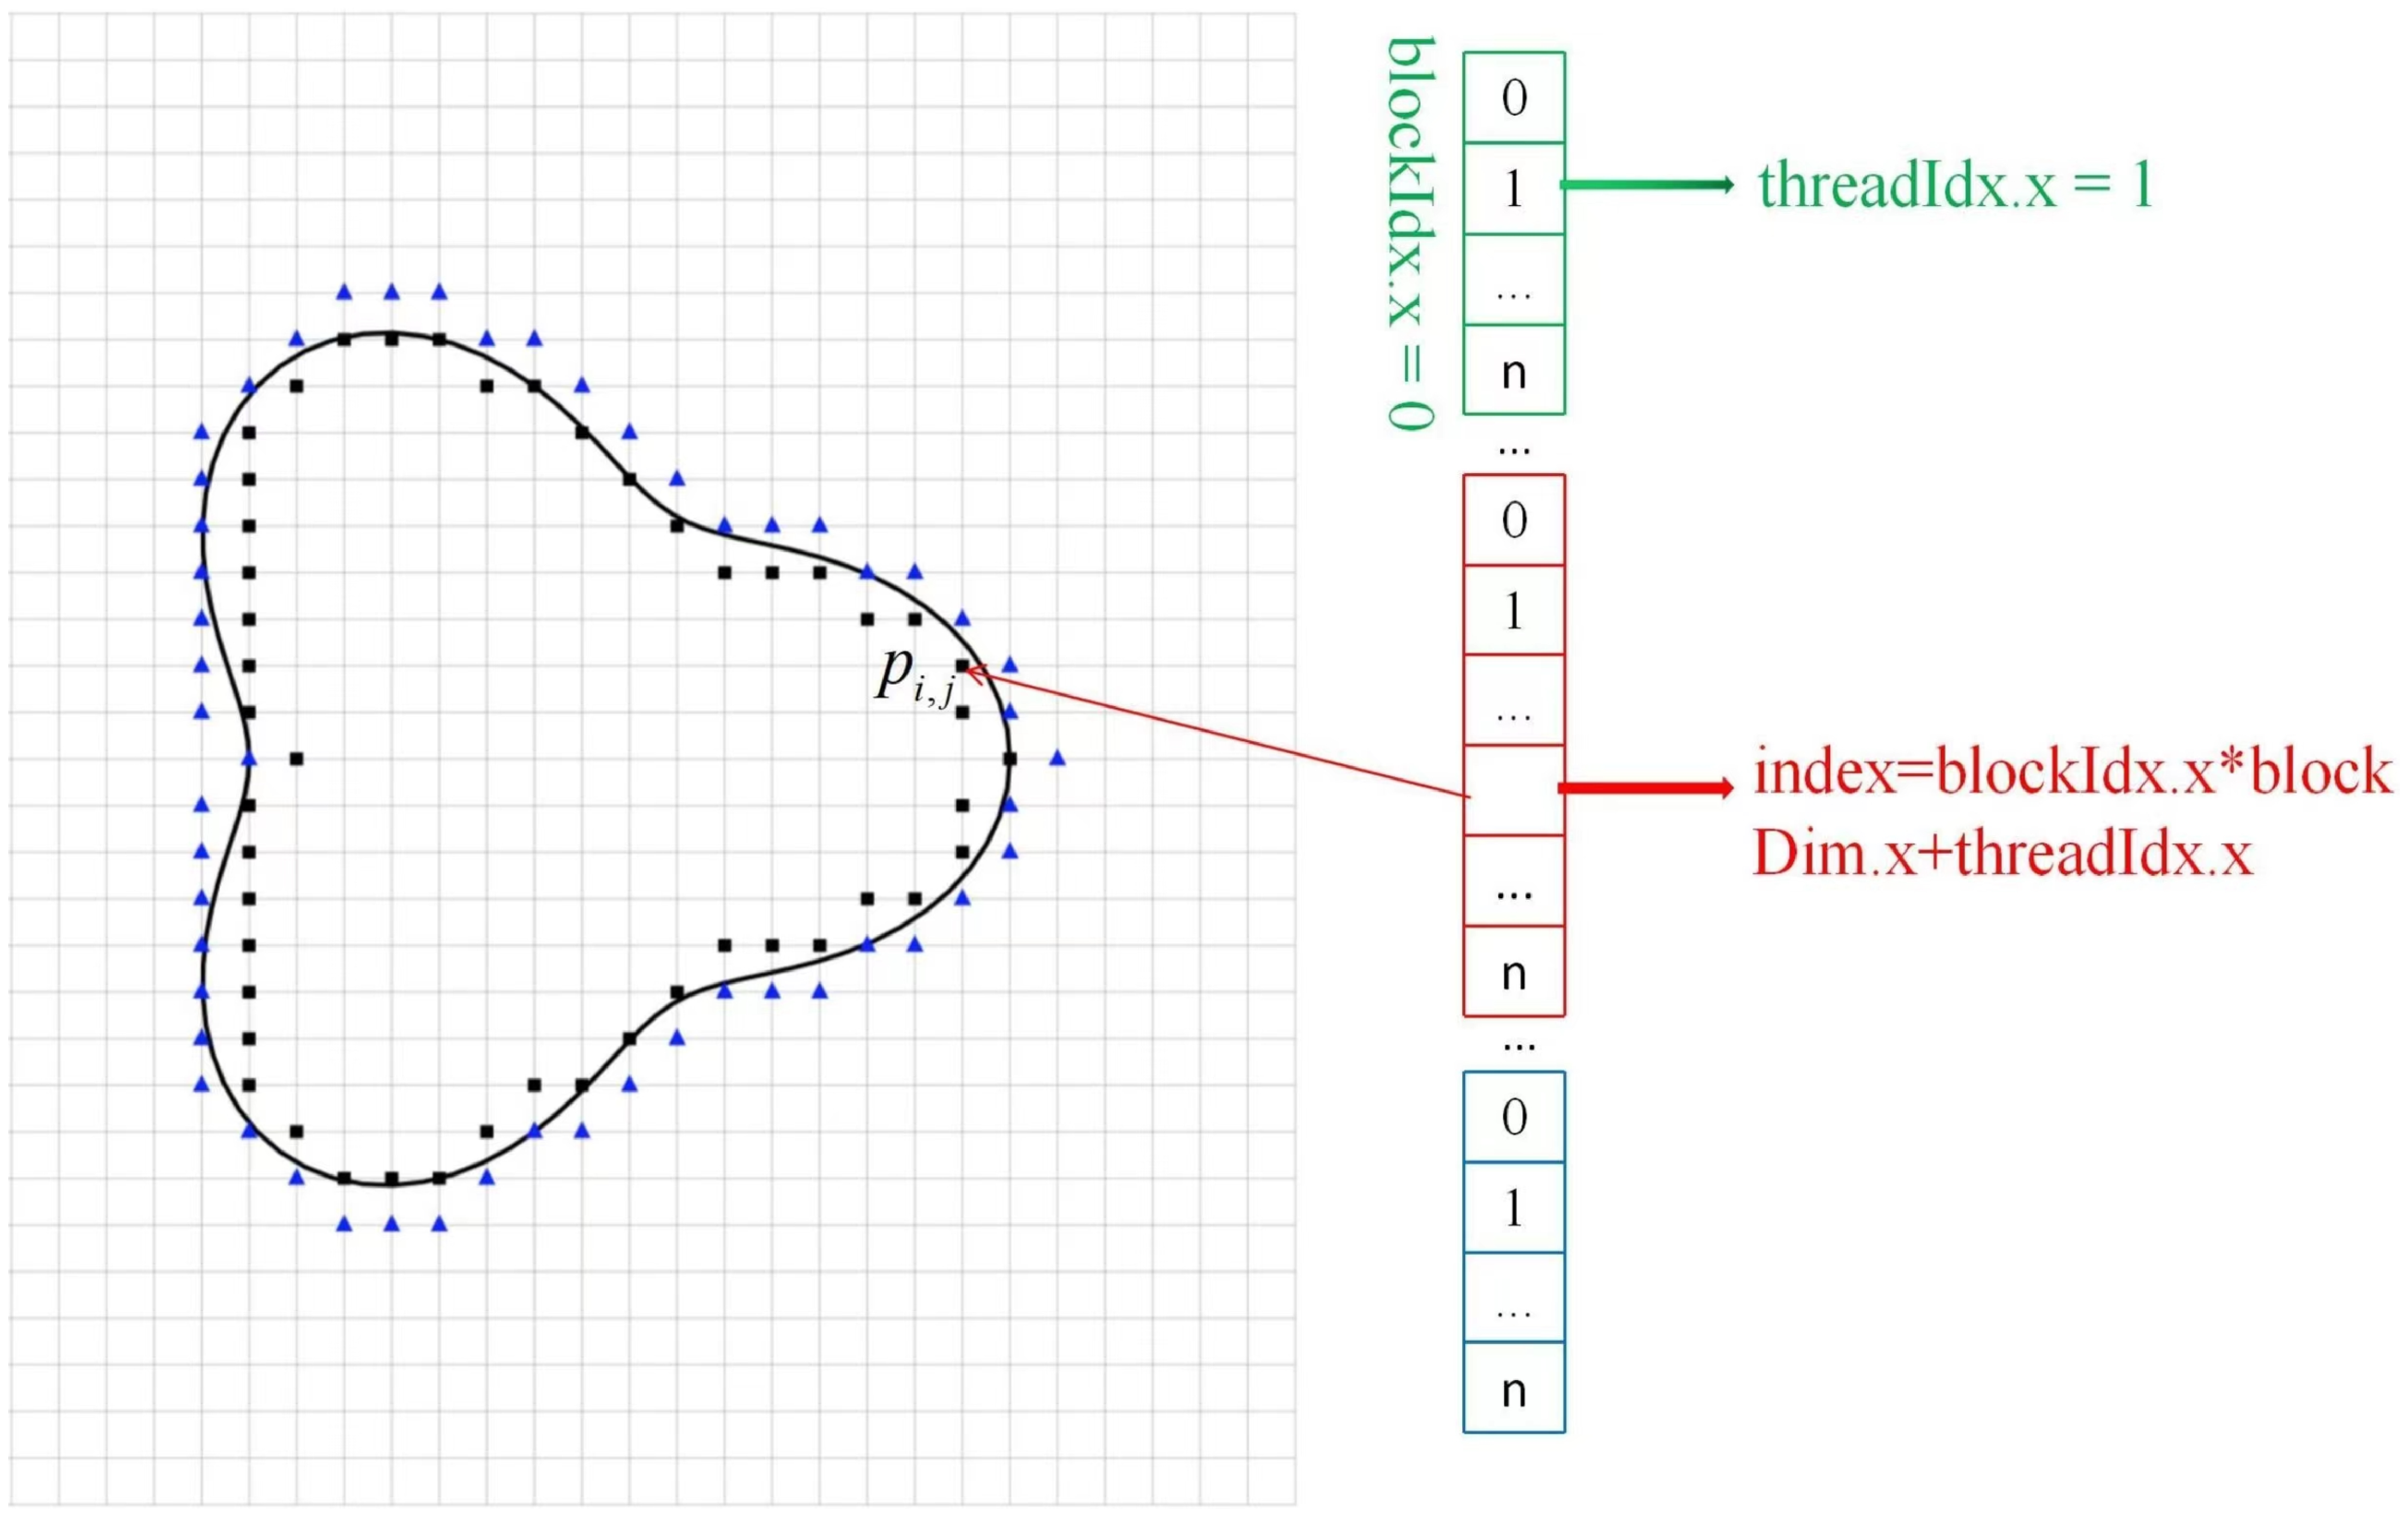
\includegraphics[width=0.56\textwidth, height=0.402\textwidth]{figure/one_gpu_irregular_node_2.eps}\label{fig:oneGPU:irregular_node}}
    \caption{A graphical scheme for intersection nodes $\ref{fig:oneGPU:intersect_node}$ and irregular nodes $\ref{fig:oneGPU:irregular_node}$. In the left, pink triangles denote intersection nodes with $x$ direction while blue squares refer to intersection nodes with $y$ direction. In the right, each irregular node is controlled by one thread. Blue triangle denotes exterior irregular node while black denotes inner node.}
    \label{fig:One_GPU:irregular_node}
\end{figure}

\iffalse
For the modified Helmholtz operator $\mathcal{L} = \Delta - \kappa \mathcal{I}$ for interface problem $\eqref{one_GPU:interface}$ is approximated by five-point discrete operator $\mathcal{L}_{h}$ on Cartesian grid $\mathcal{T}_{h}$, which reads

\begin{equation}
\frac{ v(x_{i+1},y_j)+ v(x_{i-1},y_j)+ v(x_i,y_{j+1})+ v(x_i,y_{j-1})-4  v(x_i,y_j)}{h^{2}}-\kappa v(x_i,y_j)=f(x_i,y_j).
\label{five-point}
\end{equation}

Here, $v(\mathbf{x})$ is the solution to the elliptic PDEs $\eqref{one_GPU:interface}$, constrained by two interface conditions on $\Gamma$. If the right-hand side  $f(\mathbf{x})$ is sufficiently smooth, then the solution to the finite difference equation \eqref{five-point} has second-order accuracy. However, the irregular domain leads to discontinuous $\tilde{f}(\mathbf{x}), v(\mathbf{x})$ and $\partial_{\mathbf{n}}v(\mathbf{x})$ in $\eqref{one_GPU:interface}$, resulting in unignorable truncation error to maintain the second order. 
% Due to the discontinuities of the solution and the normal derivative across the interface $\Gamma$, the finite difference approximation at irregular grid nodes has more significant local truncation errors than those at regular grid nodes. 
The exact estimate is as follows
$$
\Delta v(\mathbf{p}_{i,j})-\kappa v(\mathbf{p}_{i,j}) - f(\mathbf{p}_{i,j})=\begin{cases}\mathcal{O}\left(h^{2}\right) & \text { if }\mathbf{p}_{i,j} \text { is a regular node } \\ \mathcal{O}\left(h^{-2}\right) & \text { if }\mathbf{p}_{i,j} \text { is an irregular node }\end{cases}.
$$
 In order to guarantee second-order accuracy of global solution, the local truncation error at irregular points needs to recover at least first-order accuracy\cite{On2008Beale}. The procedure of correction for each irregular node will be presented in the horizontal and vertical directions as follows. 

\begin{figure}[hbpt!]
    \centering
    \subfigure[horizontal]{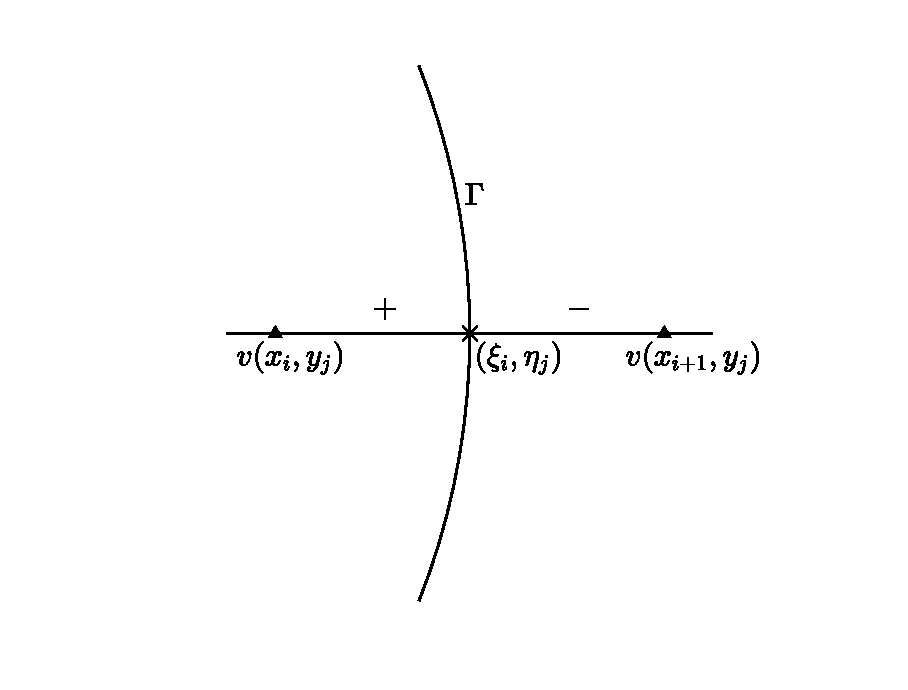
\includegraphics[scale=0.45]{figure/xinter.eps}\label{horizontal}} 
    \subfigure[vertical]{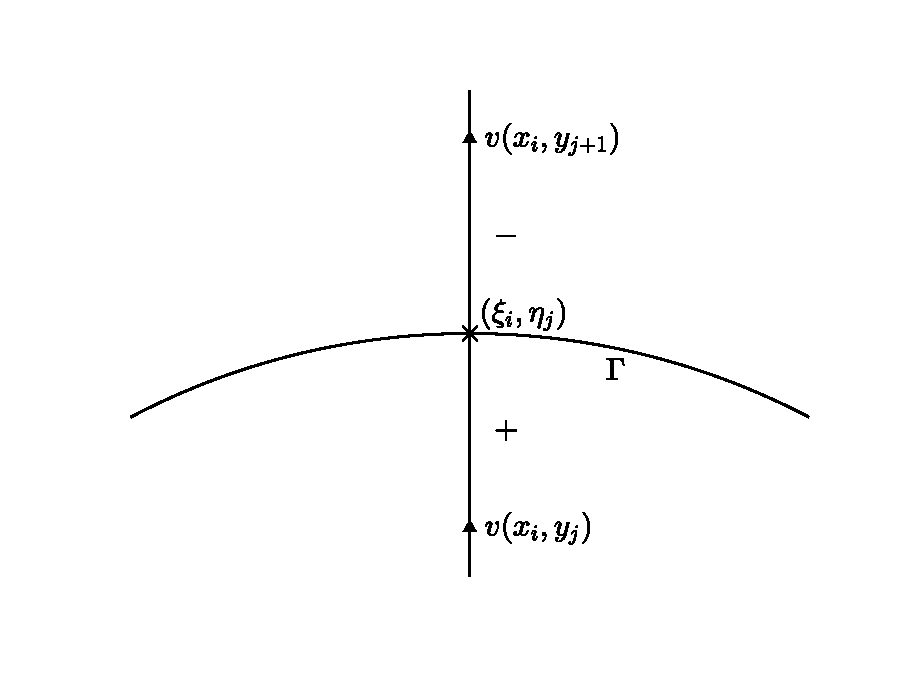
\includegraphics[scale=0.45]{figure/yinter.eps}\label{vertical}} 
    \caption{Two cases of the intersecting node in the structure grid. (a) means node lies in horizontal line while (b) implies node lies in vertical line. Triangle symbol means grid point while star symbol means intersection node of grid line. }
    \label{fig:enter-label}
\end{figure}
\noindent
$\bullet \quad \text{Horizontal direction}$
%\subsubsection{Horizontal direction}

Assuming the $\Gamma$ has an intersecting node $(\xi_{i}, \eta_{j})$ located between an exterior  node $\mathbf{p}_{i,j}$ and an interior node $\mathbf{p}_{i+1,j}$. The local truncation error of the horizontal direction can be expressed as
\begin{equation}
E_{h,x}\left(x_{i},y_{j}\right) \equiv \frac{v^{-}\left(x_{i+1},y_{j}\right)+v^{+}\left(x_{i-1},y_{j}\right)-2 v^{+}\left(x_{i},y_{j}\right)}{h^{2}}-v^{+}_{xx}\left(x_{i},y_{j}\right).
\end{equation}

According to Taylor's expansion, the horizontal part $E_{h, x}\left(x_{i}, y_{j}\right)$ of the local truncation error can be approximated by the following quantity
$$
C_{h, x}^{+}\left(x_{i}, y_{j}\right) \equiv -\frac{1}{h^{2}}\left\{[v]+\left[v_{x}\right]\left(x_{i+1}-\xi_{i}\right)+\frac{1}{2}\left[v_{x x}\right]\left(x_{i+1}-\xi_{i}\right)^{2}\right\} + H.O.T,
$$

which introduces a first-order error, since
$$
E_{h, x}\left(x_{i}, y_{j}\right)=C_{h}^{+}\left(x_{i}, y_{j}\right)+\mathcal{O}(h).
$$

The correction term $C^{+}_{h}(x_{i}, y_{j})$ depends on jumps $[v], [v_{x}]$ and $[v_{x x}]$. As a matter of fact, the jumps of partial derivatives of the function $v$ can be deduced from the interface problem $\eqref{one_GPU:interface}$. Details of the calculation of jumps are presented in the Appendix A. Similarly, $C^{-}_{h,x}(x_{i}, y_{j})$ denotes the correction of the node $\mathbf{p}_{i,j} \in \Omega^{c}$ locating near the interface $\Gamma$:
$$
C_{h, x}^{-}\left(x_{i+1}, y_{j}\right) \equiv \frac{1}{h^{2}}\left\{[v]+\left[v_{x}\right]\left(x_{i}-\xi_{i}\right)+\frac{1}{2}\left[v_{x x}\right]\left(x_{i}-\xi_{i}\right)^{2}\right\} + H.O.T.
$$

\noindent 
$\bullet \quad \text{Vertical direction}$
%\subsubsection{Vertical direction}

Assume the $\Gamma$ has an intersecting node $(\xi_{i}, \eta_{j})$ located between an exterior  node $\mathbf{p}_{i,j}$ and an interior node $\mathbf{p}_{i,j+1}$. The local truncation error of the vertical direction can be expressed as follows
\begin{equation}
E_{h,y}\left(x_{i},y_{j}\right) \equiv \frac{v^{-}\left(x_{i},y_{j+1}\right)+v^{+}\left(x_{i},y_{j-1}\right)-2 v^{+}\left(x_{i},y_{j}\right)}{h^{2}}-v^{+}_{yy}\left(x_{i},y_{j}\right).
\end{equation}

According to Taylor's expansion, the vertical part $E_{h, y}\left(x_{i}, y_{j}\right)$ of the local truncation error can be approximated by the following quantity
$$
C_{h, y}^{+}\left(x_{i}, y_{j}\right) \equiv -\frac{1}{h^{2}}\left\{[v]+\left[v_{y}\right]\left(y_{j+1}-\eta_{j}\right)+\frac{1}{2}\left[v_{y y}\right]\left(y_{j+1}-\eta_{j}\right)^{2}\right\} + H.O.T.
$$

which introduces a first-order error, since
$$
E_{h, y}\left(x_{i}, y_{j}\right)=C_{h, y}^{+}\left(x_{i}, y_{j}\right)+\mathcal{O}(h).
$$

Same to $E_{h, x}(x_{i}, y_{j})$, $E_{h, y}(x_{i}, y_{j})$ also depends on jumps of $[v]$ and $[v_{y}]$. $C^{-}_{h,y}(x_{i}, y_{j})$ denotes the correction of the node $\mathbf{p}(x_{i}, y_{j}) \in \Omega^{c}$ locating near the interface $\Gamma$
$$
C_{h, y}^{-}\left(x_{i}, y_{j}\right) \equiv \frac{1}{h^{2}}\left\{[v]+\left[v_{y}\right]\left(y_{j}-\eta_{j}\right)+\frac{1}{2}\left[v_{y y}\right]\left(y_{j}-\eta_{j}\right)^{2}\right\} + H.O.T.
$$
Therefore, the modified system becomes 
\begin{equation}
    \mathcal{L}_{h}v_{h}(\mathbf{p}_{i,j}) = \begin{cases}
    0, & \mathbf{p}_{i,j} \text{ is regular node} \\
    C^{\pm}_{h}(\mathbf{p}_{i,j}), & \mathbf{p}_{i,j} \text{ is irregular node} \end{cases}.
\end{equation}
\fi
\subsection{Interpolation} \label{one_GPU:interpolation}
% Let $v_{h}^{+}, v_{h}^{-}$ be the approximate solution of $v^{+}, v^{-}$ respectively. Assume approximate solution $v_{h}(\mathbf{x})$ is a piecewise smooth function although only the value defined at grid nodes of $\mathcal{T}_{h}$ are known. Assume the solution $v_{h}(\mathbf{x})$ is smooth in $\mathcal{B}\setminus \Gamma$. 

Fig.$\ref{interpolate}$ shows the six-point stencil of interpolated point $\mathbf{z}_{k}$ located in the shadow region of a grid cell. The stencil consists of 6 points and can be obtained by rotation or reflection transformation if $\mathbf{z}_{k}$ in another grid cell. As shown in Fig.$\ref{interpolate}$, $\mathbf{p}_{i,j}$ are the grid points for extracting value at a point $\mathbf{z}_{k} \in \Gamma$. The corresponding algorithm can be described in Algorithm $\ref{one_GPU:interpolation_algo}$:
\begin{figure}[hbpt!]
    \centering
    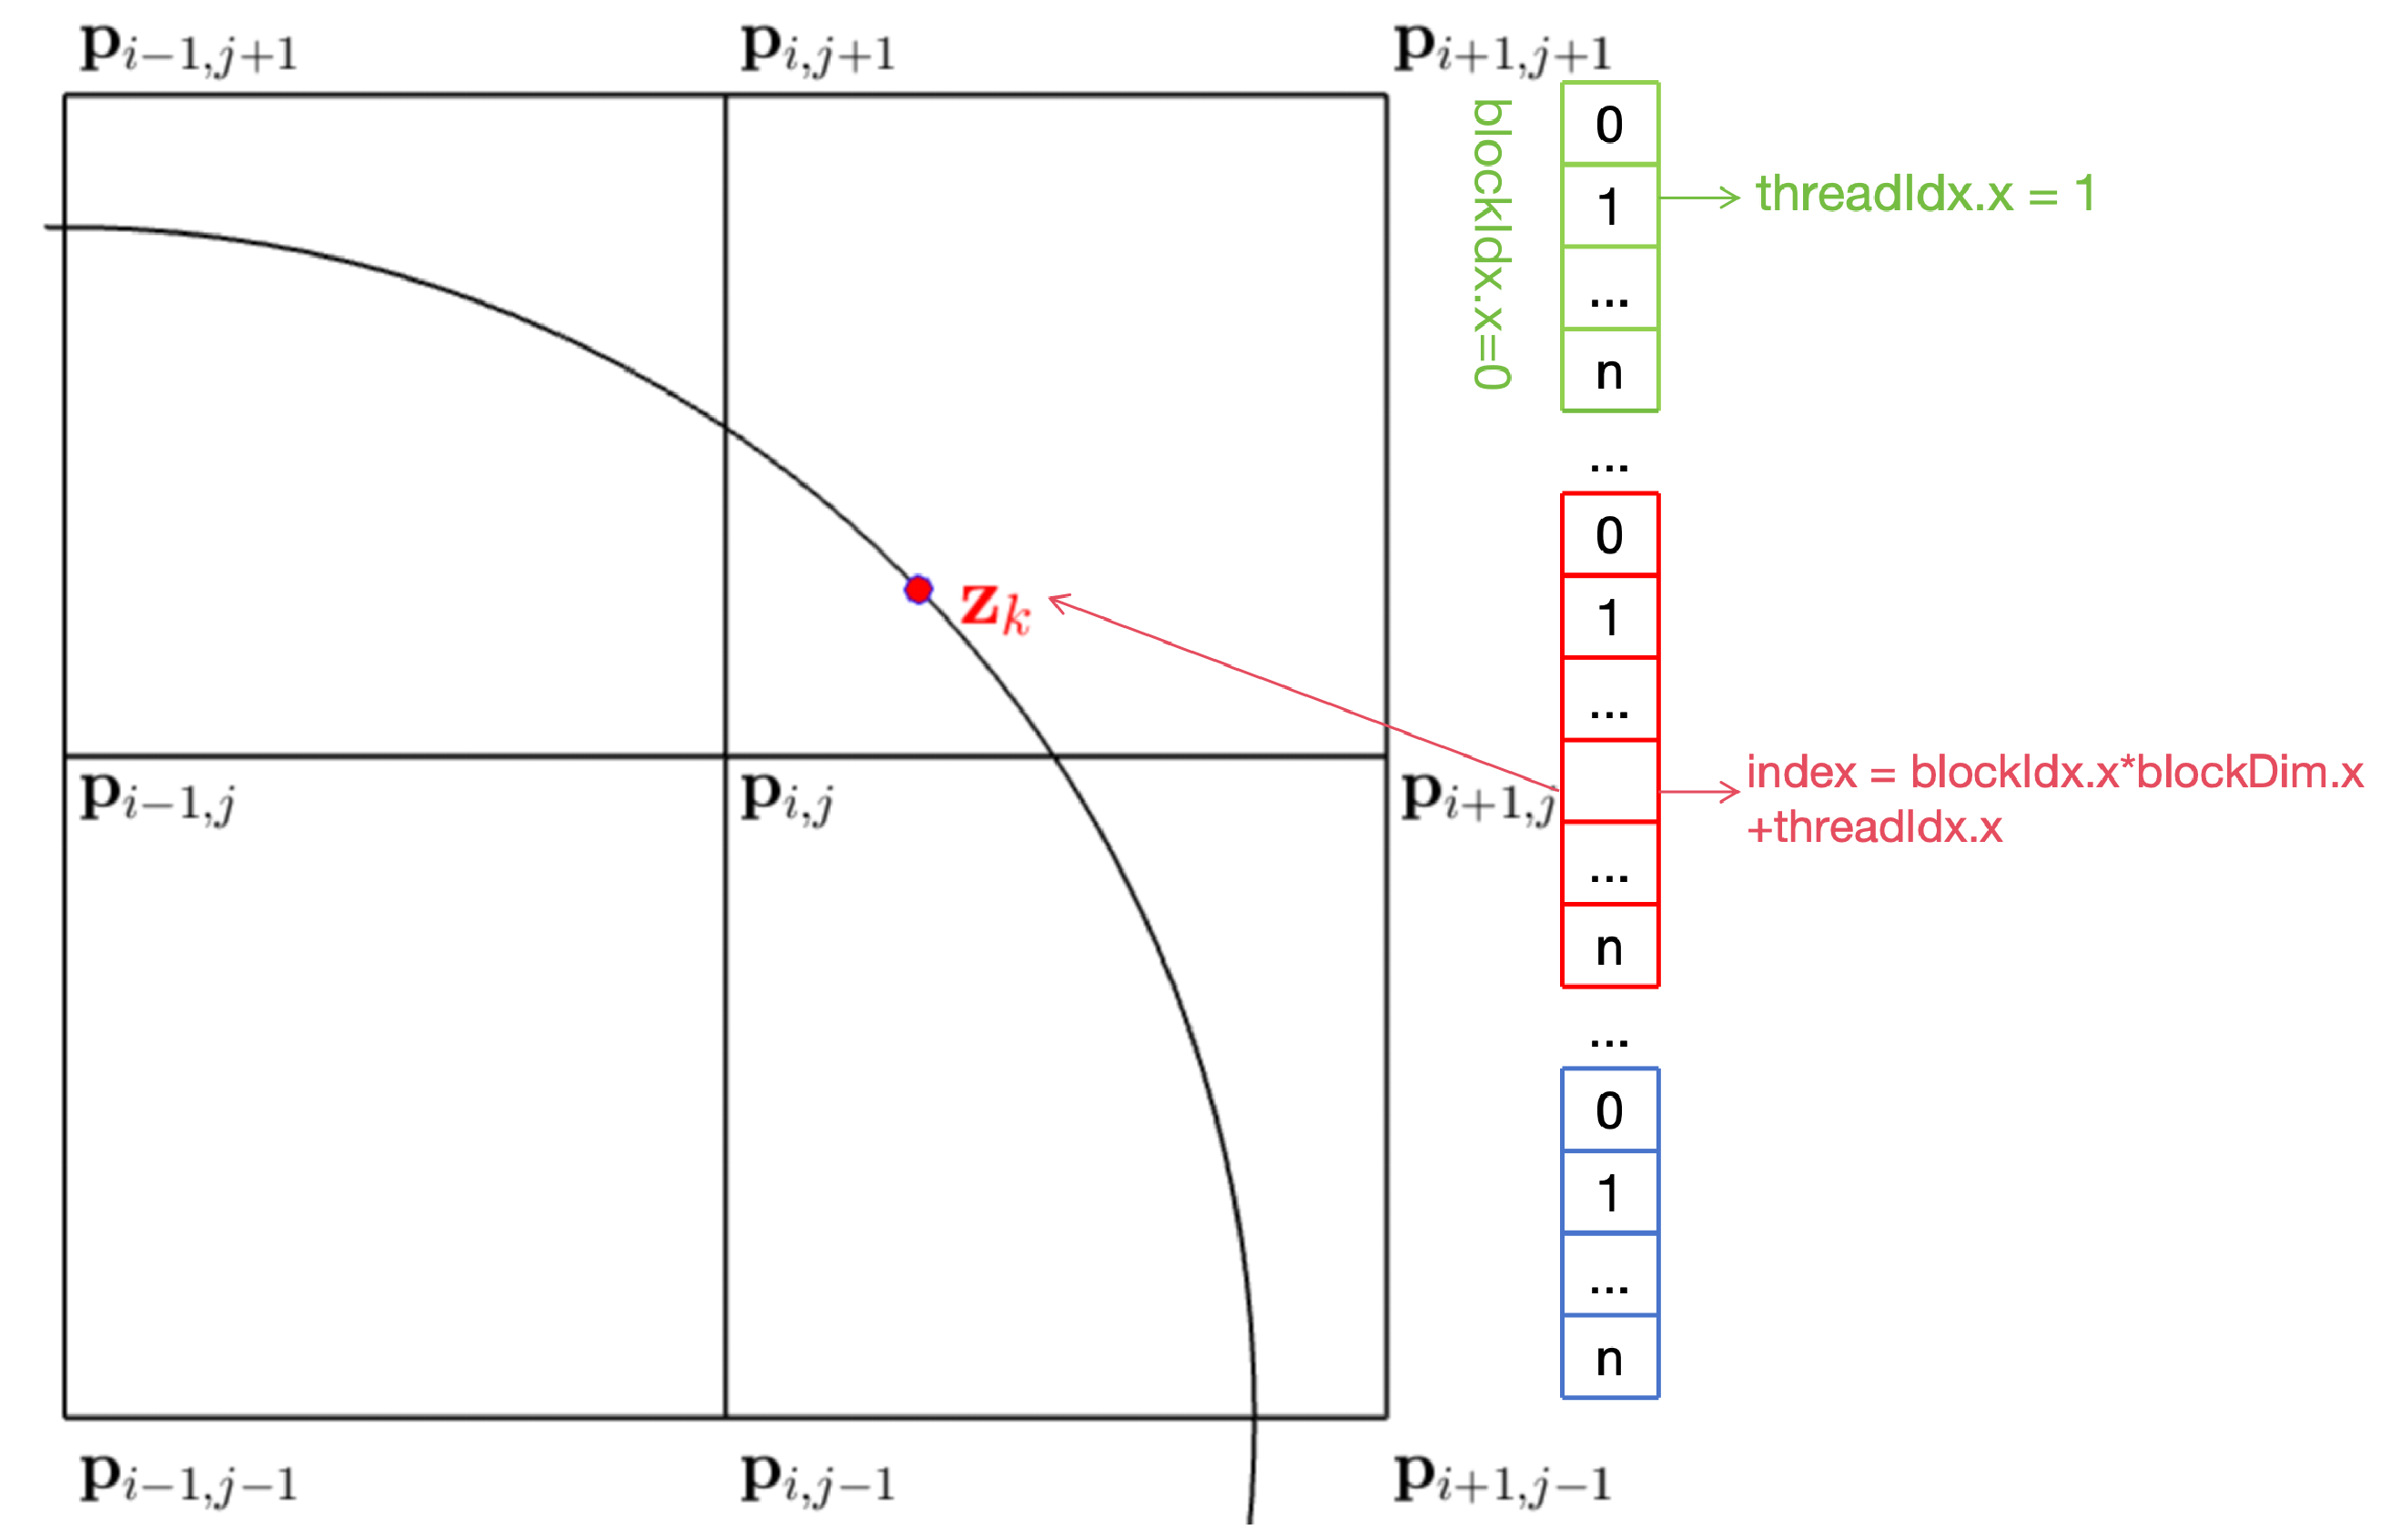
\includegraphics[width = 0.62\linewidth]{figure/one_gpu_interpolate_new2.eps}
    \caption{Interpolation schematic diagram. The evaluation of the control node $z_{k}$ depends on neighbor grid value $\mathbf{p}_{I,J}, I = \left\{i-1, i, i+1\right\}, J = \left\{j-1, j, j+1\right\}$. For parallelization, every control node is controlled by one thread. }
    \label{interpolate}
\end{figure}
\iffalse
As shown in Fig.$\ref{interpolate}$, $\mathbf{p}_{i,j}$ are the grid points for extracting value of a point $\mathbf{z}_{k} \in \Gamma$. Following the notations, let $(\xi_{i}, \eta_{j}) = \mathbf{p}_{i,j} - \mathbf{z}_{k}$, thanks to Taylor expansion of $v_{h}(\mathbf{z}_{k})$ at boundary node $\mathbf{x}$:
\begin{equation}
    \begin{aligned}
    v_{h}(\mathbf{p}_{i,j}) & = v_{h}^{+}(\mathbf{z}_{k})+ \frac{\partial v_{h}^{+}}{\partial x}(\mathbf{z}_{k})\xi_{i} + \frac{\partial v_{h}^{+}}{\partial y}(\mathbf{z}_{k}) \eta_{j} + \frac{1}{2}\frac{\partial^{2} v_{h}^{+}}{\partial x^{2}}(\mathbf{z}_{k})\xi_{i}^{2}\\
    & + \frac{\partial^{2} v_{h}^{+}}{\partial x \partial y}(\mathbf{z}_{k})\xi_{i}\eta_{j} + \frac{1}{2}\frac{\partial^{2} v_{h}^{+}}{\partial y^{2}}(\mathbf{z}_{k})\eta_{j}^{2} + O(|\mathbf{p}_{i,j} - \mathbf{z}_{k}|^{3}), \quad \mathbf{p}_{i,j} \in \Omega, \\
    v(\mathbf{p}_{i,j}) & = v_{h}^{-}(\mathbf{z}_{k})+ \frac{\partial v_{h}^{-}}{\partial x}(\mathbf{z}_{k})\xi_{i} + \frac{\partial v_{h}^{-}}{\partial y}(\mathbf{z}_{k}) \eta_{j} + \frac{1}{2}\frac{\partial^{2} v_{h}^{-}}{\partial x^{2}}(\mathbf{z}_{k})\xi_{i}^{2}\\
    & + \frac{\partial^{2} v_{h}^{-}}{\partial x \partial y}(\mathbf{z}_{k})\xi_{i}\eta_{j} + \frac{1}{2}\frac{\partial^{2} v_{h}^{-}}{\partial y^{2}}(\mathbf{z}_{k})\eta_{j}^{2} + O(|\mathbf{p}_{i,j} - \mathbf{z}_{k}|^{3}), \quad \mathbf{p}_{i,j} \in \Omega^{c}. \label{interpolate2}
    \end{aligned}
\end{equation}

In order to be concise, we denote the limit value at $\mathbf{z}_{k} \in \Gamma$ of the $v_{h}$ and its derivatives are denoted as
\begin{equation}
\begin{aligned}
    V^{\pm} & = v_{h}^{\pm}(\mathbf{z}_{k}), \quad V_{x}^{\pm} = \frac{\partial v_{h}^{\pm}}{\partial x}(\mathbf{z}_{k}), \quad V_{y}^{\pm} = \frac{\partial v_{h}^{\pm}}{\partial y}(\mathbf{z}_{k}). \\
    V_{xx}^{\pm} & = \frac{\partial^{2} v_{h}^{\pm}}{\partial x^{2}}(\mathbf{z}_{k}), \quad V_{xy}^{\pm} = \frac{\partial^{2} v_{h}^{+}}{\partial x\partial y}(\mathbf{z}_{k}), \quad V_{yy}^{\pm} = \frac{\partial^{2} v_{h}^{+}}{\partial y^{2}}(\mathbf{z}_{k}).
\end{aligned}\label{one_GPU:substitude}
\end{equation}

Let $V_{i,j}$ be $v_h({\mathbf{p}_{i,j}})$. Substituting $\eqref{one_GPU:substitude}$ into $\eqref{interpolate2}$ yields
\begin{equation}
\begin{aligned}
    & V^{+}+V_x^{+} \xi_j+V_y^{+} \eta_j+\frac{1}{2} \xi_j^2 V_{x x}^{+}+\frac{1}{2} \eta_j^2 V_{y y}^{+}+\xi_j \eta_j V_{x y}^{+}=V_{i,j}, \quad \mathbf{p}_{i,j} \in \Omega, \\
    & V^{-}+V_x^{-} \xi_j+V_y^{-} \eta_j+\frac{1}{2} \xi_j^2 V_{x x}^{-}+\frac{1}{2} \eta_j^2 V_{y y}^{-}+\xi_j \eta_j V_{x y}^{-}=V_{i,j}, 
    \quad \mathbf{p}_{i,j} \in \Omega^{c}.
\end{aligned}\label{one_GPU:substep}
\end{equation}
Let 
\begin{equation}
    J_{i,j} = [V] + [V_{x}]\xi_{i} + [V_{y}]\eta_{j} + \frac{1}{2}[V_{x x}]\xi_{i}^{2} + [V_{x y}] \xi_{i} \eta_{j} + \frac{1}{2}[V_{y y}]\eta_{j}^{2}, \quad \mathbf{p}_{i,j} \in \Omega^{c},
\end{equation}
thus the expansion $\eqref{interpolate2}$ can be reinterpreted as follows:
\begin{equation}
    V_{i,j}+ J_{i,j} =  V^{+} + V_{x}^{+}\xi_{i} + V_{y}^{+}\eta_{j}+ \frac{1}{2}V^{+}_{x x}\xi_{i}^{2} + 
    V_{x y}^{+}\xi_{i}\eta_{j} + \frac{1}{2}V^{+}_{y y}\eta_{j}^{2}, \quad \mathbf{p}_{i,j} \in \Omega^{c}.
\end{equation}
As a result, a 6x6 linear system is formed and is non-singular. The new variables can be solved by a simple direct method such as QR decomposition or LU decomposition. 
The corresponding algorithm can be described in Algorithm $\ref{one_GPU:interpolation_algo}$:
\fi
\begin{algorithm}
\renewcommand{\algorithmicrequire}{\textbf{Input:}}
\renewcommand{\algorithmicensure}{\textbf{Output:}}
\caption{Interpolation Procedure}
\begin{algorithmic}[1]
\Require $\text{intersection nodes, irregular nodes, } \Phi, \mathcal{F}$.
\Ensure $\text{the value and its derivatives at control node $\mathbf{z}_{k}$}$.
\State Locate index of control nodes by $\text{index} \xleftarrow[]{}$ blockIdx.x $\times$ blockDim.x + blockIdx.x.
\For {\text{control node $\mathbf{z}_{k} \in \Gamma$}: }
    \State Compute corresponding jumps of value and its derivatives respectively.
    \State Find interpolate stencil and formulate interpolate linear system.
    \State Solve linear system and extract the boundary data on $\mathbf{z}_{k}$.
\EndFor 
\end{algorithmic}\label{one_GPU:interpolation_algo}
\end{algorithm}

\subsection{GMRES iteration with FFT-based solver} \label{one_GPU:solver} 
$\bullet \textbf{ FFT-based solver }$
% \begin{algorithm}[h!]
% \renewcommand{\algorithmicrequire}{\mathbf{Input:}}
% \renewcommand{\algorithmicensure}{\mathbf{Output:}}
% \caption{GMRES method}
% \begin{algorithmic}[1]
% \Require $\text{corrected value} \tilde{f}_{i,j}$.
% \Ensure $\text{the value of}$ $v_{i,j}$.
% \While {convergence}
%     \State \textcolor{red}{$r_{0} = \hat{g}_{D} - \mathcal{K}_{D} \varphi$}
%     \State \textcolor{blue}{$\beta = ||r_{0}||_{2}$}
%     \State \textcolor{green}{$\mu_{1} = \frac{r_{0}}{\beta}$}
%     \For{$j = 1$ to $m$} 
%         \State \textcolor{red}{$w_{j} = \mathcal{K}_{D}\mu_{j}$}
%         \For {$i = 1$ to $j$}
%             \State \textcolor{cyan}{$h_{i,j} = (w_{j}, \mu_{i}$)}
%             \State \textcolor{purple}{$w_{j} = w_{j} - h_{i,j}\mu_{i}$}
%         \EndFor
%         \State \textcolor{blue}{$h_{j+1, j} = ||w_{j}||_{2}$}
%         \State \textcolor{green}{$\mu_{j+1} = \frac{w_{j}}{h_{j+1, j}}$}
%     \EndFor
%     \State $\text{set } M_{m} = [\mu_{1}, \cdots, \mu_{m}] \text{, and } \hat{H}_{m} = (h_{i,j}) \text{ is upper Hessenberg matrix of size } (m+1) \times m$
%     \State $\text{solve a least-square problem: } \min_{y\in \mathbf{R}^{2}}||\beta \mathbf{e}_{1} - \hat{H}_{m}y||_{2}$
%     \State \textcolor{orange}{$\varphi_{m} = \varphi_{0} + M_{m}y_{m}$}
%     \If{\textcolor{blue}{$||\hat{g}_{D} - \mathcal{K}\varphi_{m}||_{2} < \epsilon$}}
%     \State $\text{convergence = true}$
%     \EndIf
%     \State $\varphi_{0} = \varphi_{m}$
% \EndWhile
% \end{algorithmic}\label{one_GPU:GMRES_algo}
% \end{algorithm}
The most important feature of the KFBI method is the conversion of a volumn or boundary integral into an interface problem. The solution to the interface problem consists of two steps. The first step is to make corrections to ensure accuracy, and the second is to solve it using a fast algorithm, such as  FFT-based solver\cite{Wu2013}. The discrete linear system  can be solved using the FFT-based solver on GPU by implementing CUDA programming and invoking cusparse\cite{naumov2010cusparse} and cufft libraries\cite{govindaraju2008high}. The algorithm can be described as 
Algorithm $\ref{one_GPU:FFT_algo}$:
\begin{algorithm}[ht]
\renewcommand{\algorithmicrequire}{\textbf{Input:}}
\renewcommand{\algorithmicensure}{\textbf{Output:}}
\caption{FFT-based solver of modified Helmholtz equation in GPU}
\begin{algorithmic}[1]
\Require $\text{corrected value}~\tilde{f}_{i,j}$.
\Ensure $\text{the solution of interface problem:} $ $v_{i,j}$.
\State Take the FFT transform on the $\tilde{f}_{i,j}$ on $y$-dimension and get transformed $\hat{\tilde{f}}_{i, j}$.
\State Solve tridiagonal linear system with right hand side term $\hat{\tilde{f}}_{i, j}$, and get solution $\hat{v}_{i, j}$. 
\State Take the inverse FFT transform on $\hat{v}_{i, j}$ on $y$-dimension, and get final solution $v_{i,j}$.
\end{algorithmic}\label{one_GPU:FFT_algo}
\end{algorithm}

In Algorithm $\ref{one_GPU:FFT_algo}$, it should be pointed out that FFT transforms depend on the boundary condition on $\partial \mathcal{B}$. If $\partial \mathcal{B}$ is the periodic, Dirichlet or Neumann, one needs to do periodic, Fast Sine Transform(FST), or Fast Cosine Transform(FCT), respectively. There is no difference in the influence of the results in the three scenarios. However, in this paper, we perform FFT on one dimension and solve the tridiagonal resulting system on another, which is the fastest and most efficient. \\
$\bullet \textbf{ GMRES iteration }$ GMRES is an iterative method for solving nonsymmetric linear systems. The method aims to approximate the solution by the vector in a Krylov subspace with minimal residual. The condition number of BIE $\eqref{one_GPU:second_fredholm}$ is relatively small, allowing for fast convergence of GMRES iteration \cite{saad2003iterative}. 

%Numerical experiment shows that compared to Richardson iteration, using GMRES to solve equation $\eqref{one_GPU:modified_helmholtz} $will require fewer iterations and therefore achieve faster convergence speed \cite{ying2013kernel, ying2014kernel, xie2019fourth}.

% Sometimes, GMRES does not converge or requires too many iterations to meet the convergence criteria. Therefore, in most cases, GMRES must include a preconditioning step to improve its convergence. 

From $\eqref{one_GPU:richardson1}$, we denote  : 
\begin{align}
    \mathcal{K}_{D}(\varphi)(\mathbf{x}) & := (\frac{1}{2}I + W)(\varphi)(\mathbf{x}), \quad \mathbf{x} \in \Gamma
\end{align}
\begin{algorithm}[ht]
\renewcommand{\algorithmicrequire}{\textbf{Input:}}
\renewcommand{\algorithmicensure}{\textbf{Output:}}
\caption{GMRES with restarts in GPU}
\begin{algorithmic}[1]
\Require $\text{corrected value} ~\tilde{f}_{i,j}$.
\Ensure $\text{the solution of BIE}($\ref{one_GPU:second_fredholm}): $\varphi_{m}$.
\State convergence = false
\While {convergence == false}
    \State $r_{0} = \hat{g}_{D} - \mathcal{K}_{D} \varphi$
    \State $\beta = ||r_{0}||_{2}$
    \State $\mu_{1} = \frac{r_{0}}{\beta}$
    \For{$j = 1$ to $m$} 
        \State $w_{j} = \mathcal{K}_{D}\mu_{j}$
        \For {$i = 1$ to $j$}
            \State $h_{i,j} = (w_{j}, \mu_{i}$)
            \State $w_{j} = w_{j} - h_{i,j}\mu_{i}$
        \EndFor
        \State $h_{j+1, j} = ||w_{j}||_{2}$
        \State $\mu_{j+1} = \frac{w_{j}}{h_{j+1, j}}$
    \EndFor
    \State $\text{Set } M_{m} = [\mu_{1}, \cdots, \mu_{m}] \text{, and } \hat{H}_{m} = (h_{i,j}) \text{ is upper Hessenberg matrix of order } (m+1) \times m$
    \State $\text{Solve a least-square problem: } \min_{y\in \mathbf{R}^{2}}||\beta \mathbf{e}_{1} - \hat{H}_{m}y||_{2}$
    \State $\varphi_{m} = \varphi_{0} + M_{m}y_{m}$
    \If{$||\hat{g}_{D} - \mathcal{K}\varphi_{m}||_{2} < \epsilon$}
    \State $\text{convergence = true}$
    \EndIf
    \State $\varphi_{0} = \varphi_{m}$
\EndWhile
\end{algorithmic}\label{one_GPU:GMRES_algo}
\end{algorithm}
The main points of the GMRES method with restarts are presented in Algorithm $\ref{one_GPU:GMRES_algo}$. It is worth noting that the matrix-vector product in GMRES is replaced by the KFBI method(line 2 and 6). As for computing vector norm(line 3, 11, and 17), inner product(line 8), scalar-vector operation(line 4 and 12), and some axpy operation(line 9), they are implemented by the cuda kernel functions. Since the calculated $\varphi$ need to be reintegrated into the next iteration, the GPU information needs to be transferred back to the CPU after each GMRES iteration to obtain updated $M_{m-1}$ to $M_{m}$(line 14). Therefore, the calculations for the least squares method are also performed on the CPU(line 15).